\chapter{Stochastic Tractography Algorithm}
\begin{figure}
  \center 
	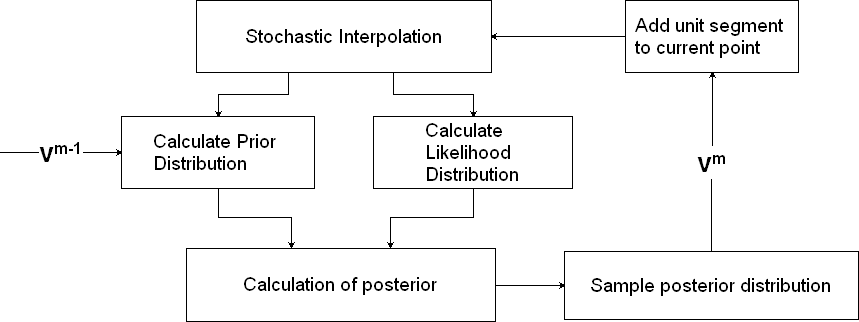
\includegraphics[width=\linewidth]{stflowsmall}
	\caption{A flow chart demonstrating key steps in the stochastic tractography algorithm}
	 \label{fig:stflow}
\end{figure}
The stochastic tractography algorithm implemented in this thesis is based on Friman's \cite{frimanTMI06} approach with some modifications to the stopping criteria.  Figure \ref{fig:stflow} provides a flow chart demonstrating key steps in the algorithm. 

A fiber tract is modeled as a sequence of unit vectors.  The orientation of these unit vectors is determined by sampling a posterior fiber orientation distribution which is dependent on the local diffusion data as well as the orientation of the unit vector in the previous step.  The posterior distribution is a normalized product of the prior likelihood of the fiber orientation and the likelihood of that fiber orientation given the local diffusion data.

Friman uses a subset of the tensor model which is called a constrained diffusion model.  In this model, the two smallest eigenvectors of diffusion tensor are equal, constraining the shape of the diffusion tensor to be linearly anisotropic.  The constrained model rules out the possibility of nonlinear, or non-cylindrical anisotropic diffusion distributions.  Deviations from linearly anisotropic diffusion distributions are captured as uncertainty in the fiber orientation.  The constrained model is combined with a Gaussian DWI noise model to obtain a fiber orientation likelihood function.  The parameters for the constrained model are derived from a weighted least squares estimation of the parameters for the log tensor model.

The orientation of each vector depends only on the previous vector.  This dependency is formulated in the prior on the fiber orientation.  Prior knowledge about the regularity of the fiber tract can encoded in this prior probability.  The prior also serves to prevent the fiber from backtracking, since the likelihood distribution alone is axially symmetric.

Friman's approach is a Bayesian inference algorithm similar to Behrens's but with some important optimizations \cite{frimanTMI06}.  In contrast with Behrens's two-compartment observation model, the constrained model used by Friman is derived from the thoroughly studied tensor model of diffusion.  The advantage of using the constrained model is that it is relatively easy to estimate the parameters for the model.  The parameters for the constrained model are obtained after the tensor model has been fit to the diffusion data.  Since the parameters for the tensor model are easily obtained through many computationally efficient ways, the constrained model's parameters are likewise easy to obtain.  The constrained model can be fit to every voxel within a matter of seconds whereas Behrens's model takes a couple of hours \cite{frimanTMI06}.  Additionally Friman avoids using MCMC techniques by assuming that parameters other than the principle diffusion direction take on their ML estimates with certainty within each voxel.  Friman demonstrates that eliminating this source of uncertainty has little effect on the resulting posterior fiber orientation distribution.

In Friman's paper on stochastic tractography, the tracking is terminated when an encountered voxel's diffusion distribution below a minimal measure of anisotropy.  However, since the stochastic tractography algorithm takes into account this uncertainty with an increase in the spatial variance of sampled fibers, this termination criterion seems arbitrary and contradictory with the goals of stochastic tractography, which is to enable sampling of tracts in regions of uncertainty.  Thus we replace this termination criterion with one which terminates tractography based on the posterior probability that a fiber tract exists within the current voxel.  The posterior probability that a fiber tract exists in a given voxel can be obtained by performing a soft segmentation of white matter on an anatomical image co-registered with the DWI data.  Alternatively, the soft segmentation can also be performed on the B0 image of the DWI data set, thus eliminating the need for additional data.  While this may seem equivalent to using an anisotropy threshold criterion, since white matter generally has higher anisotropy than gray matter, it does not exclude regions of white matter which have low anisotropy due to crossing fibers.  This criteria should enable the algorithm to detect more tracts than under the anisotropy termination criteria.

\section{Mathematical Derivation}
%insert the theorem which finds the closest constrained model here
\subsection{Linearized Diffusion Tensor Model}
For each voxel in the DWI volume a signal intensity $z_i$ can be measured given a particular diffusion weighting factor $b_i$ and magnetic gradient direction $\mathbf{g}_{i}=(g_{ix} \quad g_{iy} \quad g_{iz})^T$.  The subscript $i$ enumerates multiple measurements of the same voxel under different magnetic gradient directions.

%insert tensor model reference below
The tensor model is a popular model used to describe the relationship between a particular gradient direction $\mathbf{g}_i$, the diffusion weighting factor $b_i$ and the measured voxel intensity $z_i$:  
%
%
\begin{equation} \label{eq:tensormodel}
z_{i}=z_0 e^{-b_i \mathbf{g}_i^T \mathbf{D} \mathbf{g}_i}
\end{equation}


\begin{equation} \label{eq:Dtensor}
\mathbf{D}=
\left( \begin{array}{ccc}
D_{xx} & D_{xy} & D_{xz} \\
D_{xy} & D_{yy} & D_{yz} \\
D_{xz} & D_{yz} & D_{zz} \\
\end{array} \right)
\end{equation}
%
%
where $\mathbf{D}$ is the diffusion tensor, encoded as a $3\times3$ matrix that describes the rate of diffusion in 3D space.  


Taking the log of both sides of the equation leads to a more tractable linear relationship:

\begin{equation} \label{eq:logtensormodel}
\log(z_i)=\log(z_0)-b_i \mathbf{g}_i^T \mathbf{D} \mathbf{g}_i
\end{equation}
%
%
The model is now in a linear form so that we can apply standard techniques such as least squares to estimate the diffusion parameters (the entries of the $\mathbf{D}$).  The linearized form can be further simplified by expanding the matrix multiplications and isolating the parameters into a separate vector.

\begin{equation} \label{eq:logtensormodelexpanded}
\log(z_i)=\mathbf{a}_i^T\mathbf{q}
\end{equation}

\begin{equation} \label{eq:xi}
\mathbf{a}_i=
\left( \begin{array}{ccccccc}
1 & -b_ig_{ix}^2 & -b_ig_{iy}^2 & -b_ig_{iz}^2 & -2b_ig_{ix}g_{iy} & -2b_ig_{ix}g_{iz} & -2b_ig_{iy}g_{iz}
\end{array} \right)^T
\end{equation}


\begin{equation} \label{eq:q}
\mathbf{q}=
\left( \begin{array}{ccccccc}
z_0 & D_{xx} & D_{yy} & D_{zz} & D_{xy} & D_{xz} & D_{yz}
\end{array} \right)^T
\end{equation}
%
%
The entries of the diffusion tensor $\mathbf{D}$ and the scaling factor $z_0$ now correspond to entries in the $\mathbf{q}$ vector.

There are 7 parameters that must be solved for in $\mathbf{q}$.  At least 6 additional independent equations are required in order to solve for the parameters.  These equations can be obtained by measuring the voxel intensity using at least 7 noncolinear gradient directions $g_i$ and optionally by varying the diffusion weighting factor $b_i$.  However, more than 7 directions are required to estimate the variance of the original data, as we discuss later in this section. The full system of equations containing all $n$ measurements of a voxel can be succinctly represented in matrix form:
\begin{equation} \label{eq:fulllogtensor}
\log(\mathbf{z})=\mathbf{A}\mathbf{q}
\end{equation}
Where $\mathbf{A}$ is a $n\times7$ matrix and $\log(\mathbf{z})$ is an $n$ length vector of the $n$ voxel intensities.  The least squares solution has the following form:

%include the Gram-Schmidtt optimization
\begin{equation} \label{eq:LSUpsilon}
\hat{\mathbf{q}} = (\mathbf{A}^T\mathbf{A})^{-1}\mathbf{A}^T\log(\mathbf{z})
\end{equation}

\subsection{Constrained Diffusion Tensor Model}
Although the tensor model provides a good description of a general diffusion profile, ultimately we would like to estimate the distribution of the fiber orientations from the voxel intensities.  To simplify the tractography process we assume that each voxel contains only one fiber, and the majority of diffusion occurs in the single direction dictated by this single fiber.  The assumption is mathematically modeled by constraining the diffusion tensor to forcing the two smallest eigenvalues to be equal.  Under this constraint the eigen-decomposition of the diffusion tensor $\mathbf{D}$

\begin{equation} \label{eq:EigenD}
\mathbf{D} = \lambda_1 \mathbf{\hat{e_1}}\mathbf{\hat{e_1}}^T + 
\lambda_2 \mathbf{\hat{e_2}}\mathbf{\hat{e_2}}^T +
\lambda_3 \mathbf{\hat{e_3}}\mathbf{\hat{e_3}}^T
\end{equation}
%
%
is simplified by assuming the two smallest eigenvalues $\lambda_2 = \lambda_3 = \alpha $:

% a little confused about the expression below
\begin{eqnarray} \label{eq:ConstrainedEigenD}
\mathbf{D} & = & \lambda_1 \mathbf{\hat{e_1}}\mathbf{\hat{e_1}}^T +
\alpha (\mathbf{\hat{e_2}}\mathbf{\hat{e_2}}^T + \mathbf{\hat{e_3}}\mathbf{\hat{e_3}}^T) \nonumber\\
& = & (\lambda_1 - \alpha) \mathbf{\hat{e_1}}\mathbf{\hat{e_1}}^T + \alpha\mathbf{I} \nonumber\\
& = & \beta\mathbf{\hat{e_1}}\mathbf{\hat{e_1}}^T + \alpha\mathbf{I}
\end{eqnarray}
%
%
Substituting this expression into the tensor model in equation(\ref{eq:tensormodel}) yields the constrained model:

\begin{equation} \label{eq:ConstrainedModel}
z_{i} = z_0 e^{-\alpha b_i} e^{-\beta b_i (g_i^T\mathbf{\hat{v}} ) ^2}
\end{equation}
%
%
where $\mathbf{\hat{v}}$ represents $\mathbf{\hat{e_1}}$, the eigenvector associated with the largest eigenvalue.  This change emphasizes that the constrained model attempts to model the underlying fiber orientation and not the general diffusion profile.

The parameters of the constrained model can be derived from the parameters of the tensor model.  Given matrix $\mathbf{D}$ with the eigenvalue factorization of equation (\ref{eq:EigenD}), the closest symmetric matrix, in terms of the Frobenius norm , with the two equal smallest eigenvalues is \cite{frimanTMI06}:

\begin{equation} \label{eq:derivedmatrix}
\mathbf{S} = \lambda_1 \mathbf{\hat{e_1}}\mathbf{\hat{e_1}}^T + 
\frac{\lambda_2 + \lambda_3}{2} (\mathbf{\hat{e_2}}\mathbf{\hat{e_2}}^T +
\mathbf{\hat{e_3}}\mathbf{\hat{e_3}}^T)
\end{equation}
%
%
Hence after fitting the tensor model we obtain the constrained model parameters:

\begin{equation} \label{eq:constrainedparams}
\alpha = \frac{\lambda_2 + \lambda_3}{2},\;
\beta = \lambda_1 - \alpha,\;
\mathbf{\hat{v}} = \mathbf{\hat{e}}
\end{equation}

The additional constraints imposed by the constrained model reduces the goodness of fit, as compared to the diffusion tensor model, for voxels that do not exhibit anisotropic diffusion.  The reduction in anisotropy may be due to partial volume effects and the constrained model captures this uncertainty with an increase residual variance which translates into a wider fiber orientation likelihood function.

\subsection{Fiber Orientation Likelihood Function}

The log of the measured voxel intensity can be described as the log of the true intensity $z_i$ with some additive noise $\epsilon$:

\begin{equation} \label{eq:logsignal}
y_i = \log(z_i) + \epsilon_i
\end{equation}
%
%
For moderate levels of SNR, Salvador et al. \cite{salvador} demonstrates that the distribution of the noise (\ref{eq:logsignal}) is approximately normal with a mean of zero and a variance equal to the variance of the original complex data \cite{salvador}, divided by the square of the non-log noise-free voxel intensity:

\begin{equation} \label{eq:noisepdf}
p(\epsilon_i) = N \left( 0, \frac{\sigma_i^2}{z_i^2} \right)
\end{equation}
%
%
Therefore the resultant distribution of the log of the measured voxel intensity can be modeled by the same normal distribution, whose mean has been shifted by the log of the noise-free intensity:
\begin{equation} \label{eq:signalpdf}
p(y_i) = N\left( \log(z_i), \frac{\sigma_i^2}{z_i^2} \right)
\end{equation}
%
%
%An additional assumption must be made that the n measurements are independent, is this reasonable?
The joint distribution of the $n$ noisy voxel log-intensities is obtained by multiplying the $n$ distributions together.  It is assumed that the variance of the original complex data is constant across all $n$ measurements of a voxel.

\begin{equation} \label{eq:jointsignalpdf}
p(\mathbf{y}) = \prod_{i=1}^{n}N\left( \log(z_i), \frac{\sigma^2}{z_i^2} \right)
\end{equation}

In other words, equation (\ref{eq:jointsignalpdf}) is the likelihood of observing the measured data given the noise-free intensities $z_i$.  Since we cannot directly observe $z_i$ we estimate them by fitting parameters for the constrained model from the observed noisy data $\mathbf{y}$.  Hence, after substituting in the constrained model, $z_i$ becomes $\hat{z}_i$ and equation (\ref{eq:jointsignalpdf}) becomes the likelihood of observing the measured data given a choice of parameters for the constrained model.  Since the parameter of primary interest is the estimated fiber direction $\mathbf{\hat{v}}$, it is separated from the estimated secondary parameters $\mathbf{\hat{\theta}} = \{\hat{z}_0, \hat{\alpha}, \hat{\beta}, \hat{\sigma}^2\}$.  $\sigma^2$ is the variance of the original complex data \cite{salvador}, not the variance of the intensity $z_i$.  It can be estimated by calculating the residual variance after fitting the parameters of the constrained model.

%change this to use weighted least squares estimation
\begin{equation} \label{eq:ResVar}
\hat{\sigma}^2 = \frac{(\log(\mathbf{y})-\mathbf{A}\hat{\mathbf{q}})^T(\log(\mathbf{y})-\mathbf{A}\hat{\mathbf{q}})}{n - 7}
\end{equation}

\begin{equation} \label{eq:likelihood}
p(\mathbf{y}|\mathbf{\hat{v}},\mathbf{\hat{\theta}}) = \prod_{i=1}^{n}N\left( \log(\hat{z}_i), \frac{\hat{\sigma}^2}{\hat{z}_i^2} \right)
\end{equation}



\subsection{Connectivity Probability Function}
%To generate a fiber tract we must randomly select a fiber orientation probability density distribution 
%The distribution of primary interest is the the posterior distribution of the fiber orientation in a voxel given the data and the previous 
% given a choice for the parameters of the model ($\alpha, \beta, \mathbf{v}$)
% Voxels whose diffusion deviates significantly from the assumption that there exists only one primary direction of diffusion will exhibit a large residual variance.  This residual variance communicates information regarding the uncertainty of fiber orientation due to noise as well partial volume effects (crossing fibers).
 
A generated fiber tract $k$ of length $l$ can be modeled as string of $l$ unit vectors lined end to end: $\mathbf{v}_{k, 1:l} = \{\mathbf{\hat{v}}_1,\ldots,\mathbf{\hat{v}}_l\}_k$.  $\Omega_A^l$ is the set of all possible $l$ length paths that originate from point A.  A probability function can be defined on the path space for $l$ length paths: $p(\mathbf{v}_{k, 1:l})$ and consequently $p(\Omega_A^l)=1$.  Additionally, a discrete probability function $p(l)$ can be defined on the path length.
Given the diffusion measurements $\mathbf{y}$, the probability that region $A$ is connected to region $B$ by a fiber tract, assuming that the path length is independent of the diffusion measurements is:
\begin{equation} \label{eq:connectivity}
p(A\rightarrow B|\mathbf{y}) = \sum_{l=1}^{\infty} \int_{\Omega_{AB}^n}p(l)p(\mathbf{v}_{1:l}|\mathbf{y})
\end{equation}

In general, equations such as (\ref{eq:connectivity}) which contain multidimensional integrals over complex path spaces are not tractable analytically and must be calculated numerically.  The equations below provide a method to approximate equation (\ref{eq:connectivity}) numerically.  $N_l$ paths of length $l$ are sampled from the path space $\Omega_A^l$.  $\mathbb{I}$ is an indicator function that takes on the value 1 only if a particular $l$ length path $\mathbf{v}_{1:l}^k$ originating from region A passes through region B, and is 0 otherwise.  The indicator function is used to calculate the fraction of sampled paths originating in region A that pass through B, of a particular length $l$.  Finally, these fractions are weighted by the probability of the path length $p(l)$ and summed over all possible path lengths.  The infinite summation over path length converges because there is a maximum path length beyond which longer lengths have zero probability.

\begin{equation} \label{eq:indicator}
\mathbb{I} = \left\{ \begin{array}{ll}
	1 & \mathbf{v}_{k, 1:l} \in \Omega_{AB}^n \\
	0 & \textrm{otherwise}
	\end{array} \right.
\end{equation}

\begin{equation} \label{eq:numconnectivity}
p(A\rightarrow B|Y) \approx \sum_{l=1}^\infty \sum_{k=1}^{N_n} p(l) \frac{\mathbb{I}(\mathbf{v}_{k,1:l})}{N_n}
\end{equation}

\subsection{Stochastic Fiber Tract Generation}
According to equation (\ref{eq:numconnectivity}), we must randomly sample tracts originating from region $A$.  These tracts can be generated stochastically, in the sense that the tract can be generated from repeated samples from a probability distribution.  In this case we are drawing from the distribution of fiber orientations at a given point in space.  This prior distribution can be refined by incorporating likelihood information from the constrained model, as well as prior information regarding the regularity of the fiber tract, to generate a posterior fiber orientation distribution.

\begin{equation} \label{eq:posterior}
p({\mathbf{\hat{v}}_i, \theta | \mathbf{\hat{v}}_{i-1}, \mathbf{y}}) =
\frac {p(\mathbf{y}| \mathbf{\hat{v}}_{i-1}, \mathbf{\hat{v}}_i, \theta) p(\mathbf{\hat{v}}_i, \theta | \mathbf{\hat{v}}_{i-1})}
{p(\mathbf{y}|\mathbf{\hat{v}}_{i-1})}
\end{equation}

Assuming the secondary parameters $\theta$ at the current point are independent of the previous step direction and prior knowledge about the next step direction: $p(\mathbf{\hat{v}}_i, \theta | \mathbf{\hat{v}}_{i-1}) = p(\mathbf{\hat{v}}_i | \mathbf{\hat{v}}_{i-1})p(\theta)$ and assuming diffusion measurements at the current point don't depend on the previous step direction: $p(\mathbf{y}| \mathbf{\hat{v}}_{i-1}, \mathbf{\hat{v}}_i, \theta) = p(\mathbf{y}| \mathbf{\hat{v}}_i, \theta)$ and $p(\mathbf{y}|\mathbf{\hat{v}}_{i-1}) = p(\mathbf{y})$ equation (\ref{eq:posterior}) simplifies:
%
%
\begin{equation} \label{eq:posteriorsimp}
p({\mathbf{\hat{v}}_i, \theta | \mathbf{\hat{v}}_{i-1}, \mathbf{y}}) =
\frac {p(\mathbf{y}| \mathbf{\hat{v}}_i, \theta) p(\mathbf{\hat{v}}_i | \mathbf{\hat{v}}_{i-1}) p(\theta)}
{p(\mathbf{y})}
\end{equation}
%
%
The denominator $p(\mathbf{y})$ normalizes the posterior probability distribution, allowing it to integrate to 1, and can be written as the integral of the numerator.
%
%
\begin{equation} \label{eq:normalization}
p(\mathbf{y}) = \int_{\mathbf{\hat{v}}_i, \theta} p(\mathbf{y}| \mathbf{\hat{v}}_i, \theta) p(\mathbf{\hat{v}}_i | \mathbf{\hat{v}}_{i-1}) p(\theta)
\end{equation}
%
%
The likelihood function $p(\mathbf{y}| \mathbf{\hat{v}}_i, \theta)$ is given by equation \ref{eq:likelihood}.

The prior probability function $p(\mathbf{\hat{v}}_i | \mathbf{\hat{v}}_{i-1})$ is used to encode knowledge about the regularity of fiber tracts:
\begin{equation} \label{eq:prior}
p(\mathbf{\hat{v}}_i | \mathbf{\hat{v}}_{i-1}) = 
\frac{1}{\zeta} \left\{\begin{array}{ll}
	(\mathbf{\hat{v}}_i^T\mathbf{\hat{v}}_{i-1})^\gamma & \mathbf{\hat{v}}_i^T\mathbf{\hat{v}}_{i-1} \ge 0, \\
	0 & \mathbf{\hat{v}}_i^T\mathbf{\hat{v}}_{i-1} < 0
 \end{array} \right.
\end{equation}
While data from invasive studies nerve fibers can be used to estimate this PDF, for the purposes of this implementation a simple distribution given by (\ref{eq:prior}) where $\gamma \ge 0$ and $\frac{1}{\zeta}$ is a normalization factor that allows the distribution to integrate to 1.  This particular distribution gives preference to paths which continue in the prior direction and gives zero probability to perpendicular turns.  The most important function of the prior is to prevent the fiber tract from backtracking on itself.  Without the prior, this may occur because the likelihood function is symmetric.

Since we want to obtain the posterior PDF for the fiber direction alone, we must marginalize the joint posterior distribution (\ref{eq:posteriorsimp}) by integrating over the secondary parameters $\theta$.  To simplify this integration, we remove uncertainty regarding the secondary parameters, $\theta$ by assuming an ML estimate.  These ML estimates were calculated by fitting the constrained model (\ref{eq:constrainedparams}).  Under this assumption equation (\ref{eq:normalization}) simplifies to an integration only over the fiber directions $\mathbf{\hat{v}}_i$.  To simplify drawing samples from the posterior distribution, the continuous PDF (\ref{eq:posteriorsimp}) can by approximated by a discrete PDF as long as the continuous PDF is sampled finely enough.  Friman et al. \cite{frimanTMI06} found empirically that 2,562 directions spread evenly over a unit sphere $S$ was sufficient.  Taking these simplifications into account, equation (\ref{eq:posteriorsimp}) becomes:

\begin{equation} \label{eq:posteriordiscrete}
p(\mathbf{\hat{v}}_i|\mathbf{\hat{v}}_{i-1}, \mathbf{y}) = 
\frac{p(\mathbf{y}| \mathbf{\hat{v}}_i, \theta) p(\mathbf{\hat{v}}_i | \mathbf{\hat{v}}_{i-1})}
{\sum_{\mathbf{\hat{v}} \in \mathbf{S}} p(\mathbf{y}| \mathbf{\hat{v}}_i, \theta) p(\mathbf{\hat{v}}_i | \mathbf{\hat{v}}_{i-1})}
\end{equation}

Finally, since the probabilistic tractography is performed in the continuous space while the diffusion data is discretized, a decision must be made about which voxel's diffusion information should be used in the calculation of the posterior PDF at the current point.  This algorithm chooses an probabilistic interpolation method suggested by Behrens et al. \cite{behrensMRM03} which randomly selects a voxel near the current tract generation point, with closer voxels having a higher probability of being selected.
%talk through key portions of the math
%present a block diagram of the algorithm




%need to add in a bit about how they are different in the way they sample the PDF

%talk about how it differs from other algorithms
%talk about using incorporating the posterior probability of white matter
%talk about why we choose to segment the gray/white matter using b0 image instead of using diffusion information
